\section{Graph Summarisation}
\label{chap:summary:model}

Web Data contains a large amount of structured data spanning over many different domains, from information on movies to the description of genes. There are billions of statements and millions of entities. There is a wealth of vocabulary terms for every kind of data, which are used more or less in the way a vocabulary was design for.

In order to make sense of this deluge of data, summarisation techniques are available for different levels of the data. For example, all the information related to an entity can be summarised so to highlight the important parts. In this section, we are interested in the summarisation of the \emph{structure} of graphs. In the context of Web Data, the structure of a graph is defined by the use of predicates and classes.

We present first a model for graph summarisation in Section~\ref{sec:summary:model}. Then in Section~\ref{sec:precise-summary}, we introduce a model for a \emph{precise} summary. Finally, we emphasise the direction of \emph{approximate} graph summarisation as the only viable summarisation for Web Data in many cases in Section~\ref{sec:approximate}.% Finally, we describe how inter-linked datasets can be summarised.

\subsection{Model}
\label{sec:summary:model}

In this section, we present a formal model of graph summarisation.

\subsubsection{Properties of a Summary}

Graph summarisation is an operation over the graph that abstracts from its content, in order to highlights its structure. From a structural point of view, traversing a graph or its summary is equivalent. The summary of a graph exhibits the following properties:
\begin{enumerate}
	\item a path in the graph exists also in the summary;
	\label{sprop-path}
	\item both the graph and its summary share the same vocabulary; and
	\label{sprop-voc}
	\item a graph may conform to several summaries.
	\label{sprop-not-uniq}
\end{enumerate}
These properties of a summary are fulfilled by defining the graph summarisation as a graph \emph{homomorphism}.

\subsubsection{Graph Homomorphism}

A graph is homomorphic to another one if there exists a mapping of nodes that matches \emph{edges} from the first to the second graph. This ensures that the structure of the first graph is kept.
The Figure~\ref{fig:homomorphism} depicts two graphs, where there exists a relation $R$ that maps nodes of the left graph to nodes of the right graph. The edges of the left graph are also kept in the right graph. Indeed, there is an edge from nodes $2$ and $3$ to $1$, and as well there is an edge between their mapped nodes --- nodes $a$ and $b$ respectively.

\begin{definition}[Graph Homomorphism]
Let $G=\left\langle V, A, l_V \right\rangle$ and $\mathcal{S}=\left\langle \mathcal{W}, \mathcal{B}, l_\mathcal{W} \right\rangle$ be two graphs. Let $R \subseteq V \times \mathcal{W}$ be a binary relation.
In the context of the binary relation, $G$ is homomorphic to $\mathcal{S}$ with regards to $R$ if every edge in $G$ is \emph{mapped} to an edge in $\mathcal{S}$:
$$
\forall (u, \alpha, v) \in A\;\; \forall (x, y) \in \mathcal{W}\;\; (u, x) \in R \wedge (v, y) \in R \implies (x, \alpha, y) \in \mathcal{B}
$$
We say that $G$ is homomorphic to $\mathcal{S}$ with regards to $R$.
\end{definition}

A graph homomorphism is defined by a many-to-many binary relation $R$ from the nodes $V$ to the nodes $\mathcal{W}$, and that for every edge in $A$ there is a corresponding edge in $\mathcal{B}$. Whenever two nodes in the graph $G$ are linked by an attribute $\alpha$, then so are their corresponding nodes in the graph $\mathcal{S}$.\\

\begin{remark}
From this point on, we shall differentiate between the nodes and edges of the entity graph from those of the summary by calling a node of the summary a \emph{sumnode}, and an edge a \emph{sumedge}. Unless stated explicitly, the terms node and edge refer to the components of the entity graph.
\end{remark}

\begin{figure}
	\centering
	\usetikzlibrary{arrows}

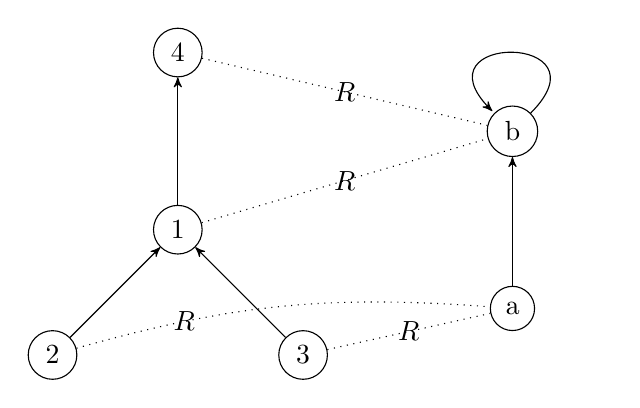
\begin{tikzpicture}[>=stealth',node distance=2.25cm]
\node [draw,circle] (1) {1};
\node [draw,circle,below left of = 1] (2) {2};
\node [draw,circle,below right of = 1] (3) {3};
\node [draw,circle,above of = 1] (4) {4};

\node [draw,circle,right of = 1,xshift=2cm,yshift=-1cm] (a) {a};
\node [draw,circle,above of = a] (b) {b};

\path (1) edge[->] (4)
		   (2) edge[->] (1)
		   (3) edge[->] (1)
		   (a) edge[->] (b)
  		   (b) edge[->,loop] (b)
		   (1) edge [dotted] node {$R$} (b)
		   (4) edge [dotted] node {$R$} (b)
		   (2) edge [dotted,bend left=10] node[near start] {$R$} (a)
		   (3) edge [dotted] node {$R$} (a);
\end{tikzpicture}
	\caption[Graph homomorphism]{Graph homomorphism. There is a relation $R$ that maps nodes of the left graph to the nodes of the right graph which keeps the connection of the right graph.}
	\label{fig:homomorphism}
\end{figure}

\paragraph{Source material.}

A graph and its summary do not share the same set of nodes. The nodes of the summary are taken from a set that is distinct from the set of nodes in the graph. We refer to that set as the \emph{source material} which we denote as $\mathcal{Z}$. We define in the following paragraphs two nodes of the summary that are used in its creation, i.e., the undefined sumnode and the sink sumnode.

\subparagraph{Undefined sumnode.}
\label{sec:undefined-sumnode}

Depending on the definition of the binary relation $R$ used in a graph homomorphism, some nodes of the graph do not have any mapping. For example, the node $v_0$ in Figure~\ref{fig:graph} does not have a $type$ edge; it has then no mapping for a summarisation relation that considers the type of a node as depicted in the Figure~\ref{fig:classes-summary}.
We map such a node of the graph to a sumnode $\mathfrak{U} \in \mathcal{Z}$ that we say to be \emph{undefined} for the binary relation $R$.

\begin{definition}[Undefined Sumnode $\mathfrak{U}$]
Let $G=\left\langle V, A, l_V \right\rangle$ and $\mathcal{S}=\left\langle \mathcal{W} \cup \{ \mathfrak{U} \}, \mathcal{B}, l_\mathcal{W} \right\rangle$ be two graphs such that $G$ is homomorphic to $\mathcal{S}$ with regards to the binary relation $R \subseteq V \times \mathcal{W}$.
Let $Q \subseteq V \times \{ \mathfrak{U} \}$ be a binary relation.
We define the sumnode $\mathfrak{U} \in \mathcal{Z}$ with $\mathfrak{U} \not \in V$ as the sumnode to which are mapped the nodes of $V$ that do not have an image in $\mathcal{W}$ as per the binary relation $R$:
$$
(u, \mathfrak{U}) \in Q \implies \not \exists x \in \mathcal{W}\; (u, x) \in R
$$
\end{definition}

A graph $G$ that is homomorphic to a graph $\mathcal{S}$ with regards to a binary relation $R$ is still the case if we add the undefined sumnode to the graph $\mathcal{S}$: we simply need to add the sumedges to the graph $\mathcal{S}$ that link to and from the undefined sumnode.

\subparagraph{Sink sumnode: content abstraction.}

The purpose of a summary is to highlight the \emph{structure} of the graph, which is defined by the properties and types. Content information does not pertain to the structure of the data, but only to individual entities. Therefore, we abstract the summary from the content in the graph, which are in general stored in sink nodes, i.e., nodes that have no outgoing edges. To do so, we map such nodes to a \emph{sink} sumnode that we identify as $\varnothing$. For example, the node labelled $Ireland$ in the Figure~\ref{fig:graph} is mapped to $\varnothing$. Also, we note that the nodes $S_2$ and $S_3$ in Figure~\ref{fig:basic-summary} are sink sumnodes.

\begin{definition}[Sink Sumnode $\varnothing$]
Let $G=\left\langle V, A, l_V \right\rangle$ and $\mathcal{S}=\left\langle \mathcal{W} \cup \{ \varnothing \}, \mathcal{B}, l_\mathcal{W} \right\rangle$ be two graphs such that $G$ is homomorphic to $\mathcal{S}$ with regards to the binary relation $R \subseteq V \times \mathcal{W}$.
Let $P \subseteq V \times \{ \varnothing \}$ be a binary relation.
We define the sink sumnode $\varnothing \in \mathcal{Z}$ with $\varnothing \not \in V$ as the sumnode to which all sink nodes in $G$ are mapped to:
$$
u \in V\; \forall \alpha \in \mathcal{L}\; \forall v \in V\; (u, \alpha, v) \not \in A \implies (u, \varnothing) \in P
$$
\label{def:sink-sumnode}
\end{definition}

\begin{remark}
	In RDF graphs, literals are mapped to the sink sumnode.
\end{remark}

\subsubsection{Graph Summary}

Given two graphs $G$ and $\mathcal{S}$, if $G$ is homomorphic to $\mathcal{S}$ with regards to a binary relation $R$, then we call $\mathcal{S}$ the summary of $G$ as per the binary relation $R$ \cite{campinas:2012:dexa}. Indeed, the summary being homomorph to $G$ retain by definition the paths in the graph described in the property~(\ref{sprop-path}). Both graph share the set of labels $\mathcal{L}$, thus meeting the property~(\ref{sprop-voc}) of a summary.

\begin{definition}[Graph Summary]
Let $V \subseteq \mathcal{Z}$ and $\mathcal{W} \subseteq \mathcal{Z}$ be two sets of nodes where $\mathcal{Z}$ is the set of source material such that
\begin{inparaenum}[(a)]
	\item $\mathcal{U} \in \mathcal{W}$;
	\item $\varnothing \in \mathcal{W}$; and
	\item $V \cap \mathcal{W} = \emptyset$.
\end{inparaenum}

Let $G=\left\langle V, A, l_V \right\rangle$ and $\mathcal{S}=\left\langle \mathcal{W}, \mathcal{B}, l_\mathcal{W} \right\rangle$ be two graphs where $l_V$ and $l_\mathcal{W}$ are two labelling functions such that $l_V : V \mapsto \mathcal{L}$ and $l_\mathcal{W} : \mathcal{W} \mapsto \mathcal{L}$; and let $R \subseteq V \times \mathcal{W}$ be a binary relation.

We call the graph $\mathcal{S}$ a summary of $G$ with respect to $R$ --- which we refer to as the \emph{summarisation relation} --- if $G$ is homomorphic to $\mathcal{S}$ with respect to $R$.
\end{definition}

Figure~\ref{fig:basic-summary} depicts a possible summary for a graph. The dotted lines illustrate the summarisation relation $R$, where we have for example $(a, S_1) \in R$ and $(John, S_3) \in R$.

\begin{figure}
	\centering
	\resizebox{.7\textwidth}{!}{
		\begin{tikzpicture}[>=stealth',->,node distance=2.5cm]
%% graph
\node[draw,circle] (a) {a};
\node[draw,circle,above left of = a,xshift=.5cm] (aage) {42};
\node[draw,circle,above right of = a,xshift=-.5cm] (aname) {John};

\node[draw,circle,below of = a] (b) {b};
\node[draw,circle,above left of = b,xshift=.5cm] (bage) {33};
\node[draw,circle,above right of = b,xshift=-.5cm] (bname) {Alice};

\coordinate (gx) at ($ (aage) + (-.75,.75) $);
\coordinate (gy) at ($ (bname) + (.95,-2.4) $);
\draw[rounded corners,dashed]  (gx) node[yshift=.3cm,xshift=1cm] {Graph $G$} rectangle (gy);

\path[every node/.style={fill=white,font=\footnotesize}]
(b) edge node {knows} (a)
(a) edge node {age} (aage)
(a) edge node {name} (aname)
(b) edge node {age} (bage)
(b) edge node {name} (bname)
;

%% summary
\node[draw,circle,right of = a,xshift=4.5cm,yshift=-1cm] (s) {$S_1$};
\node[draw,circle,above left of = s,xshift=.5cm] (sage) {$S_2$};
\node[draw,circle,above right of = s,xshift=-.5cm] (sname) {$S_3$};

\coordinate (sx) at ($ (sage) + (-.75,.75) $);
\coordinate (sy) at ($ (sname) + (.95,-3.5) $);
\draw[rounded corners,dashed]  (sx) node[yshift=.3cm,xshift=1.4cm] {Summary $\mathcal{S}$} rectangle (sy);

\path[every node/.style={font=\footnotesize}]
(s) edge[loop below] node {knows} (s)
(s) edge node[fill=white] {age} (sage)
(s) edge node[fill=white] {name} (sname)
;

\path[every node/.style={fill=white,font=\footnotesize},dotted]
(aage) edge[near end,bend right=10] node {$R$} (sage)
(bage) edge[bend left=10] node[near end] {$R$} (sage)
(aname) edge[near start,bend left=7] node {$R$} (sname)
(bname) edge node[near start] {$R$} (sname)
(a) edge[bend left=5] node {$R$} (s)
(b) edge node {$R$} (s)
;

\end{tikzpicture}
	}
	\caption[A graph and a possible summary]{A graph and a possible summary. Dotted lines labelled $R$ represent the summarisation relation that maps nodes in the graph $G$ to sumnodes in $\mathcal{S}$.}
	\label{fig:basic-summary}
\end{figure}

\paragraph{Features.}

We denote as \emph{feature} elements of the graph on which the summarisation relation is based on. As an example, attributes is a feature of the Attributes summary as defined in Definition~(\ref{def:a}).

\paragraph{Uniqueness.}

Given a summarisation relation, each node in the graph is mapped to a set of sumnodes in the summary. If the mapping is \emph{deterministic}, then there exists a unique graph summary for a graph within the context of that summarisation relation. The summarisation relations proposed in Section~\ref{sec:approximate} generate a unique summary for a given entity graph. Indeed, the conditions on which a mapping is based is deterministic. For example, the summarisation relation $R_t$ introduced in that section bases its mapping on the set of types associated to a node.

\begin{figure}
	\centering
	\begin{minipage}{.7\textwidth}
		\resizebox{\textwidth}{!}{
			\usetikzlibrary{arrows}

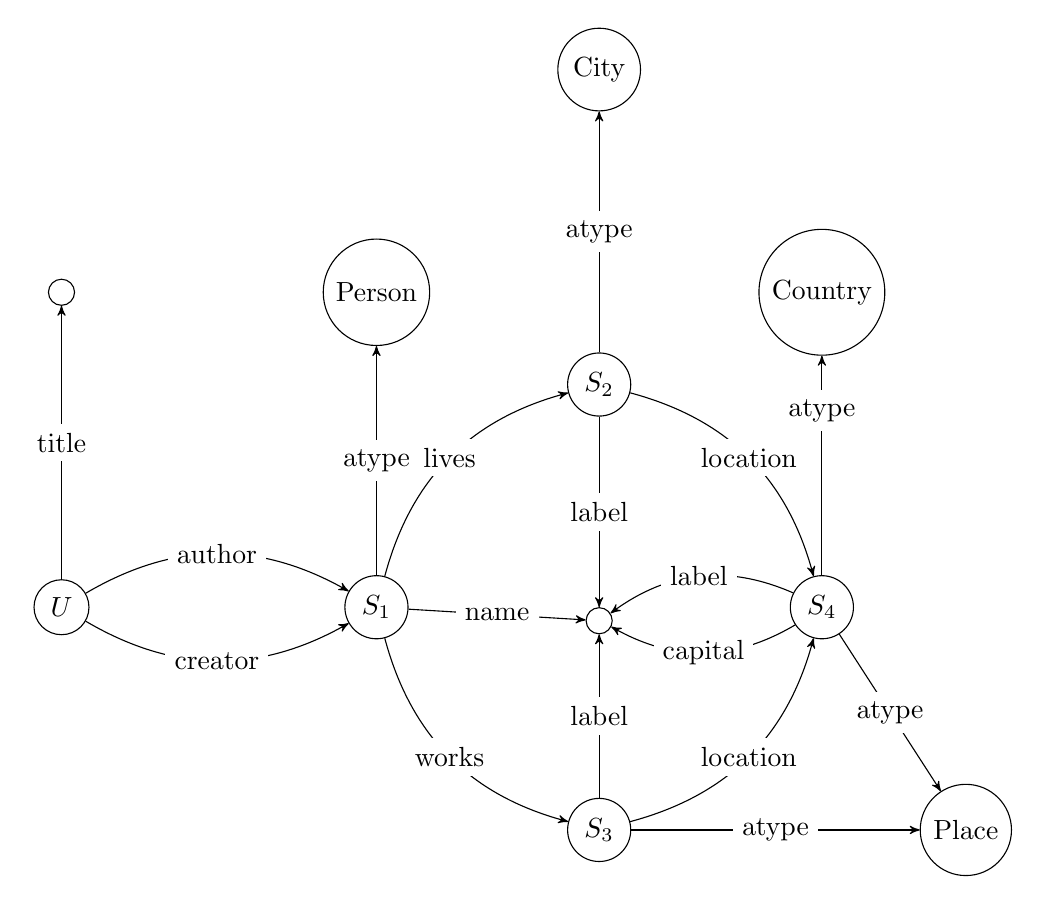
\begin{tikzpicture}[->,>=stealth',node distance=4cm]
\node [draw,circle] (b) {$\mathfrak{U}$};
\node [draw,circle,right of = b] (h1) {$S_1$};
\node [draw,circle,above right of = h1] (h2) {$S_2$};
\node [draw,circle,below right of = h1] (h3) {$S_3$};
\node [draw,circle,above right of = h3] (h4) {$S_4$};
\node [draw,circle,above of = h1] (person) {Person};
\node [draw,circle,above of = h2] (city) {City};
\node [draw,circle,above of = h4] (country) {Country};
\node [draw,circle,below right of = h4,xshift=-1cm] (place) {Place};
\node [draw,circle,above of = b] (c1) {$\varnothing$};
\node [draw,circle,below of = h2,yshift=1cm] (c2) {$\varnothing$};

\path
(b) edge node[fill=white] {title} (c1)
(h1) edge node[fill=white] {name} (c2)
(h3) edge node[fill=white] {label} (c2)
(h2) edge node[fill=white] {label} (c2)
(h4) edge[bend right] node[fill=white] {label} (c2)
(h4) edge[bend left] node[fill=white] {capital} (c2)

(h1) edge node[fill=white] {\glssymbol{atype}} (person)
(h2) edge node[fill=white] {\glssymbol{atype}} (city)
(h4) edge node[near end,fill=white] {\glssymbol{atype}} (country)
(h4) edge node[fill=white] {\glssymbol{atype}} (place)
(h3) edge node[fill=white] {\glssymbol{atype}} (place)
(h1) edge[bend left] node[fill=white] {lives} (h2)
(h1) edge[bend right] node[fill=white] {works} (h3)
(h2) edge[bend left] node[fill=white] {location} (h4)
(h3) edge[bend right] node[fill=white] {location} (h4)
(b) edge[bend right] node[fill=white] {creator} (h1)
(b) edge[bend left] node[fill=white] {author} (h1)
;
\end{tikzpicture}
		}
	\end{minipage}
	\quad
	\begin{minipage}[h]{.25\textwidth}
		\centering
		\caption*{$R_t\left(V, \mathcal{W}\right)$}
		\begin{tabular}{lc@{\hs}l}
			\toprule
			$V$ & \phantom{a} & $\mathcal{W}$ \\
			\cmidrule{1-1} \cmidrule{3-3}
			$v_0$ & \phantom{a} & $\mathfrak{U}$ \\
			$v_1$, $v_2$ & \phantom{a} & $S_1$ \\
			$v_3$ & \phantom{a} & $S_2$ \\
			$v_4$, $v_5$ & \phantom{a} & $S_3$ \\
			$v_6$, $v_7$ & \phantom{a} & $S_4$ \\
			\bottomrule
		\end{tabular}
	\end{minipage}
	\caption[Types summary of a graph]{Summary of the graph in Figure~\ref{fig:graph} with the summarisation relation $R_t$. The table indicates the mappings by $R_t$. The content in $G$ is abstracted by the sumnode $\varnothing$.}
	\label{fig:classes-summary}
\end{figure}

%We define the \emph{sink equivalence class} as the set of sink nodes, e.g., the node labelled $Ireland$ in the Figure~\ref{fig:graph} is part of this set. We remark that in the RDF data model, \emph{literals} are part of the sink equivalence class.
%\begin{definition}[Sink Equivalence Class]
%The set of sink nodes in $G$ is represented by the sink equivalence class $[\emptyset]=\left\lbrace x \in V : \not \exists (x, \alpha, y) \in A \right\rbrace$ in $G^\sim$.
%\end{definition}
%
%Depending on the $\sim$-equivalence, there can be nodes that do not have the required features to be assigned to a $\sim$-equivalence class. We define $B^\sim$ the \emph{blank $\sim$-equivalence class} as the set of such nodes of $G$, e.g., the node $v_0$ in the Figure~\ref{fig:graph} is assigned to the node $B^{\sim_t}$ in the Figure~\ref{fig:classes-summary}.
%\begin{definition}[Blank $\sim$-Equivalence Class]
%The set of nodes in $G$ for which there is no $\sim$-equivalent class is equal to the blank $\sim$-equivalence class $B^\sim$, i.e., $B^\sim=\left\lbrace x \in V : \forall y \in V, x \not \sim y \right\rbrace$.
%\end{definition}

\subsection{Precise Graph Summary}
\label{sec:precise-summary}

The purpose of a summary is to mirror the structure of the graph while being significantly smaller. Therefore, the summary can substitute the graph and improve the performance of applications. How well the summary mirrors the graph is then of high importance. From a structural perspective, a summary is precise if it is indiscernible from the entity graph, which we define in this section.

Although the structure of the graph is preserved in the summary by definition of graph homomorphism, the structure of the summary may not exactly reflect the structure of the graph. Indeed, a summary may have paths that are not present in the entity graph $G$, as depicted in the Figure~\ref{fig:homomorphism}.

Indeed, we remark that although the structure of the graph $G$ is kept in the summary, the inverse may not hold true. The Figure~\ref{fig:homomorphism} depicts a loop on the $b$ node; although there is an edge from $1$ to $4$, there is no edge in the opposite direction.\\
%In Section~\ref{chap03:sec:quality} we study the precision of an \emph{approximate} graph summary.

A summary is built from a graph based on a summarisation relation that maps each node of that graph to a sumnode, i.e., a node of the summary. An edge $(u, \alpha, v) \in A$ is mapped to a sumedge by definition of the graph homomorphism. Several paths in the graph may be mapped to a same path on the summary. We introduce the \emph{summary path instance} as the set of nodes in the graph which mappings form a path in the summary. For example, if we consider the summary in Figure~\ref{fig:classes-summary} built with the summarisation relation $R_t$, the set $\{v_1, v_3, v_6\}$ in an instance of the path $(S_1, lives, S_2) \in \mathcal{W} \wedge (S_2, lives, S_4) \in \mathcal{W}$ in that summary; indeed, we have $(v_1, S_1) \in R_t$, $(v_3, S_2) \in R_t$, and $(v_6, S_4) \in R_t$.

\begin{definition}[Summary Path Instance]
\label{def:summary-path-instance}
Let $G=\left\langle V, A, l_V \right\rangle$ be a graph, and $\mathcal{S} = \left\langle \mathcal{W}, \mathcal{B}, l_{\mathcal{W}} \right\rangle$ be the summary of $G$ according to the summarisation relation $R \subseteq V \times \mathcal{W}$.

Let $p = (x_1, \alpha_1, x_2) \in \mathcal{B} \wedge \cdots \wedge (x_n, \alpha_n, x_{n+1}) \in \mathcal{B}$ be a path in the summary $\mathcal{S}$ with $(x_1, \cdots, x_{n+1}) \in \mathcal{W}^{n+1}$.
We call the set $\{ u_1, \cdots, u_{n+1} \}$ an instance of the summary path $p$ if each node $u_i \in V$ is mapped to a sumnode $x_i$ of $p$ by the relation $R$, i.e.,:
$$
\forall i \in \left[1, n\right] \; (u_i, x_i) \in R
$$
\end{definition}

In the previous example, we remark that the summary path instance $\{v_1, v_3, v_6\}$ given for $(S_1, lives, S_2) \in \mathcal{W} \wedge (S_2, lives, S_4) \in \mathcal{W}$ in Figure~\ref{fig:classes-summary} is not the only one. Indeed, there are three more instances possible, i.e., $\{v_1, v_3, v_7\}$, $\{v_2, v_3, v_6\}$, and $\{v_2, v_3, v_7\}$. However, two out of those four do not form a path in the graph in Figure~\ref{fig:graph}, i.e., the sets $\{v_1, v_3, v_7\}$ and $\{v_2, v_3, v_7\}$. We call a summary \emph{precise} if there is no such case.

\begin{definition}[Precise Graph Summary]
\label{def:precise-summary}
Let $G=\left\langle V, A, l_V \right\rangle$ be a graph, and $\mathcal{S} = \left\langle \mathcal{W}, \mathcal{B}, l_{\mathcal{W}} \right\rangle$ be the summary of $G$ according to the summarisation relation $R \subseteq V \times \mathcal{W}$.

Let $p = (x_1, \alpha_1, x_2) \in \mathcal{B} \wedge \cdots \wedge (x_n, \alpha_n, x_{n+1}) \in \mathcal{B}$ be a path in the summary $\mathcal{S}$ with $(x_1, \cdots, x_{n+1}) \in \mathcal{W}^{n+1}$. Let the set $\{ u_1, \cdots, u_{n+1} \}$ be a summary path instance with $u_i \in V$.

We say that the summary $\mathcal{S}$ is \emph{precise} if each instance of a summary path $p$ forms a path that does exist in the graph $G$ with regards to the attributes in $p$:
$$
\forall i \in [1, n ]\; \exists \left(u_i, \alpha_i, u_{i+1} \right) \in A
$$
\end{definition}

\subsubsection{Bisimulation}
\label{chap:summary:bisim}

%\cite{Milner:1989:CC:534666} introduces the concept of bisimulation to define equivalent processes in concurrent systems. The relational coarsest partition \cite{Paige:1987:TPR:37185.37186} is generally the algorithm used for computing a bisimulation on a graph.
The bisimulation~\cite{park:1981:cai} is a notion of concurrency that studies the equality of processes.
%It can be seen as a weaker formulation of graph isomorphism in that it defines many-to-one mappings.
A bisimulation is a binary relation on $V$ that relates two nodes of the graph if itself and its inverse are \emph{simulations}.

If we consider two nodes $(u, v) \in V$, a simulation $R$ is a relation that states that for every edge $(u, \alpha, x) \in A$, there exists an edge $(v,\alpha, y) \in A$ such that there is also a simulation between the nodes $x$ and $y$. Intuitively, $(u,v) \in R$ communicates that the node $v$ can \emph{substitute} the node $u$ since all the outgoing paths from $u$ match those from $v$. A bisimulation is stronger as it states that the relation must be \emph{symmetric} as well, thus ensuring that either node may substitute the other.

Figure~\ref{fig:bisimulation} depicts the simulation relation $R$ between nodes $E_0$ and $E'_0$ such that $(E_0, E'_0) \in R$; this illustrates that:
\begin{enumerate}
	\item for every outgoing edge from $E_0$, there is also such an edge from $E'_0$; and
	\item there is a simulation between the nodes thus reached $E_i$ and $E'_i$, i.e., $(E_i, E'_i) \in R$.
\end{enumerate}
If for the node $E'_0$ the previous two points hold as well, then the binary relation $R$ is actually a \emph{bisimulation}.
%Two nodes are said \emph{bisimilar} if there is a bisimulation relation between the two.
%Sink nodes are always bisimilar.

\begin{definition}[Bisimulation]
Let $G=\left\langle V, A, l_V \right\rangle$ be a graph and $\sim \subseteq V \times V$ a binary relation on $V$.
The relation $\sim$ is a bisimulation if $\forall (x,y) \in\; \sim$:
\begin{equation*}
\forall (x, \alpha, x') \in A\; \exists (y, \alpha, y') \in A \wedge (x',y') \in\; \sim
\label{eq:b1}
\end{equation*}
The converse must hold as well, i.e.:
\begin{equation*}
\forall (y, \alpha, y') \in A\; \exists (x, \alpha, x') \in A \wedge (x',y') \in\; \sim
\label{eq:b2}
\end{equation*}
\end{definition}

\begin{remark}
Two nodes $(u, v) \in V^2$ are said \emph{bisimilar} if $(u, v) \in \sim$.
\end{remark}

\begin{figure}
	\centering
	\resizebox{.5\textwidth}{!}{
		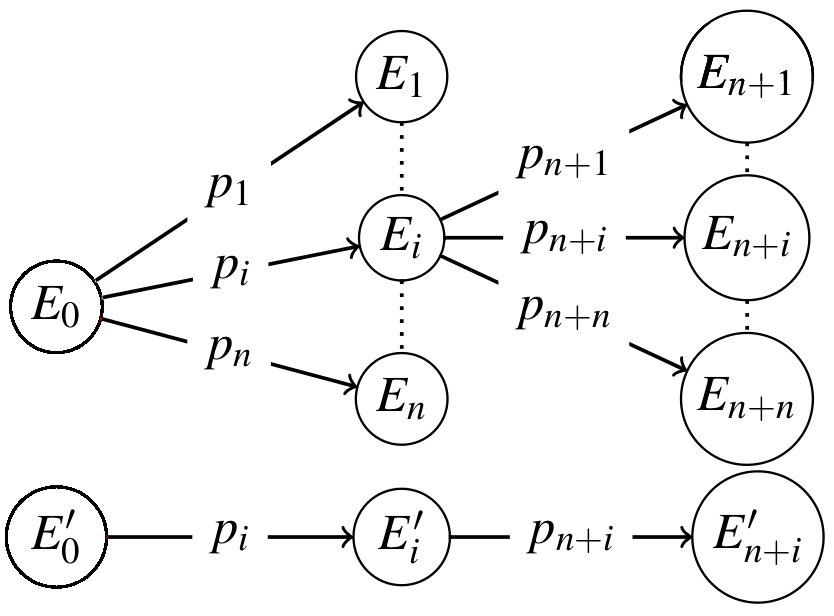
\includegraphics{04-summary/figures/bisimulation}
	}
	\caption{Simulation relation}
	\label{fig:bisimulation}
\end{figure}

The coinductive aspect of the definition ensures that two nodes are bisimilar if their \emph{outgoing} paths are the same. Kaushik et al.~\cite{kaushik:2002:cib} propose the \emph{forward-and-backward} (f\&b)-bisimulation which extends the definition by considering incoming edges in addition to the outgoing ones. Since a summary deals with the structure of the graph given by the relationships of attributes and types, we introduce the type as an additional requirement.

In addition to the requirements of a f\&b-bisimulation between two nodes, we consider their type information. We define the \emph{fbt-bisimulation} as the f\&b-bisimulation that ensures that nodes are equivalent with regards to their type as well.

\begin{definition}[FBT-Bisimulation]
Let $G=\left\langle V, A, l_V \right\rangle$ be a graph and $(\sim_f, \sim_b, \sim_t) \subseteq (V \times V)^3$ be three equivalence relations on $V$.
The relation $\approx_t \subseteq V \times V$ on $V$ is a fbt-bisimulation if $\forall (x,y) \in\; \approx_t$, we have $(x,y) \in\; \sim_f$, $(x,y) \in\; \sim_b$ and $(x,y) \in\; \sim_t$ such that:
\begin{enumerate}
\item $\sim_f$ is a forward bisimulation such that:
$$
\begin{aligned}
\forall (x, \alpha, x') \in A&\; \exists (y, \alpha, y') \in A \wedge (x',y') \in\; \sim_f \\
\text{conversely,}\;\; \forall (y, \alpha, y') \in A&\; \exists (x, \alpha, x') \in A \wedge (x',y') \in\; \sim_f
\end{aligned}
$$

\item $\sim_b$ is a backward bisimulation such that:
$$
\begin{aligned}
\forall (x^{-1}, \alpha, x) \in A&\; \exists (y^{-1}, \alpha, y) \in A \wedge (x^{-1}, y^{-1}) \in\; \sim_b \\
\text{conversely,}\;\; \forall (y^{-1}, \alpha, y) \in A&\; \exists (x^{-1}, \alpha, x) \in A \wedge (x^{-1}, y^{-1}) \in\; \sim_b
\end{aligned}
$$

\item $\sim_t$ preserves the types such that:
$$
\begin{aligned}
\forall (x, \glssymbol{atype}, t) \in A&\; \exists (y, \glssymbol{atype}, t) \in A \\
\text{conversely,}\;\; \forall (y, \glssymbol{atype}, t) \in A&\; \exists (x, \glssymbol{atype}, t) \in A
\end{aligned}
$$

\end{enumerate}
\end{definition}

\subsubsection{Bisimulation Summary}
\label{sec:bisim-summary}

Since the bisimulation is an equivalence relation, we can create equivalence classes defined as $[x] = \left\lbrace x \in V \mid y \in V,\; x \sim y \right\rbrace$; a class is the set of nodes that are bisimilar. An equivalence class is then exactly a sumnode of the summary. The summarisation relation is in this case a one-to-one mapping of the equivalence class to the sumnode.

\begin{definition}[Bisimulation Summary]
Let $G=\left\langle V, A, l_V \right\rangle$ and $\mathcal{S}_{fbt} = \left\langle \mathcal{W}_{fbt}, \mathcal{B}_{fbt}, l_{\mathcal{W}_{fbt}} \right\rangle$ be two graphs. Let $\approx_t \subseteq V \times V$ be a fbt-bisimulation relation.

The set of nodes $\mathcal{W}_{fbt} \subseteq \mathcal{Z}$ contains as many elements as there are equivalence classes as per the fbt-bisimulation relation:
$$
\lvert \mathcal{W}_{fbt} \rvert = \lvert \left\lbrace [x] \mid \exists y \in V\; x \approx_t y \right\rbrace \rvert
$$

We call $\mathcal{S}_{fbt}$ the bisimulation summary of $G$ according to the summarisation relation $R_{fbt} \subseteq V \times \mathcal{W}_{fbt}$ defined as a one-to-one mapping between the set of equivalence classes and the set $\mathcal{W}_{fbt}$:
$$
\begin{aligned}
R_{fbt} = \{ \left( u, x \right) \in V \times \mathcal{W}_{fbt} \mid & \forall v \in [u]\; \left( v, x \right) \in V \times \mathcal{W}_{fbt} \\
& \wedge \forall y \in \mathcal{W}_{fbt}\; x \neq y\; (v, y) \not \in V \times \mathcal{W}_{fbt} \}
\end{aligned}
$$
\end{definition}

\begin{remark}
We note as $R_f$ and $R_b$ the summarisation relations which equivalence classes are based on the forward $\sim_f$ and backward $\sim_b$ bisimulations, respectively.
\end{remark}

The summary depicted on the Figure~\ref{fig:fbb-summary} with the bisimulation $R_{fbt}$ assigns an equivalence class to \emph{each} node of the graph in Figure~\ref{fig:graph}. In the running example, the only difference of the summary with the entity graph is the content abstraction, e.g., the node \emph{Ireland} is represented by the node $\varnothing$.

In order to compute this summary, the algorithm proposed in \cite{Paige:1987:TPR:37185.37186} is generally used. It offers a $O\left( \vert A \vert \times log\left( \vert V \vert \right) \right)$ complexity for the computation of the bisimulation. We note that the algorithm starts from an existing partitioning of the graph. Then, the partitions are refined iteratively until all nodes in a partition are bisimilar.% The computation of the $\sim_{fbt}$-summary is achieved by applying over the $\sim_{fb}$ graph a slightly modified version of the \cite{Paige:1987:TPR:37185.37186} algorithm, in order to account for the incoming edges in the $\sim_{bb}$ definition. We remark that the complexity of all other algorithms are lower than the complexity of $\sim_{b}$.
%In addition, the \cite{Paige:1987:TPR:37185.37186} algorithm requires more than one iteration over the entity graph, the number of iterations equal to the entity graph diameter in the worst case. Iterative algorithms are sub-optimal for shared-nothing infrastructures, e.g., MapReduce. The reason is the entity graph needs to be read and written at each iteration, leading to an important IO load. Therefore, one pass algorithms can better scale to large and heterogeneous entity graphs using shared-nothing infrastructures.

\begin{figure}
	\centering
	\begin{minipage}{.75\textwidth}
		\resizebox{\textwidth}{!}{
			\usetikzlibrary{arrows}

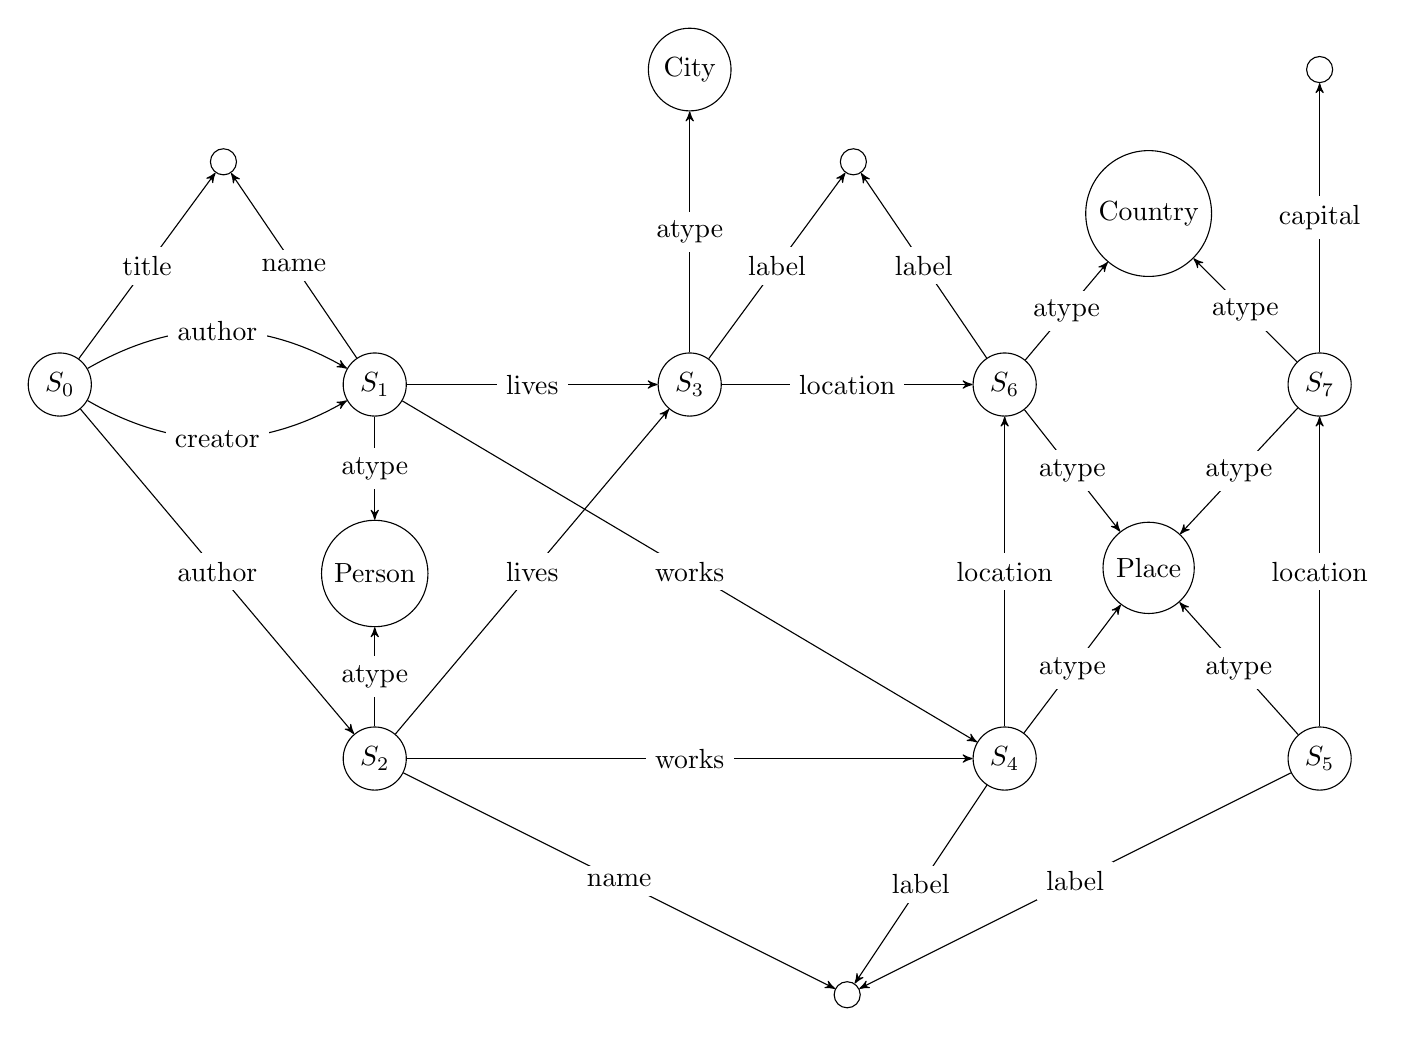
\begin{tikzpicture}[->,>=stealth',node distance=4cm]

\node [draw,circle] (n0) {$S_0$};
\node [draw,circle,right of = n0] (n1) {$S_1$};
\node [draw,circle,below of = n1,yshift=-.75cm] (n2) {$S_2$};
\node [draw,circle,right of = n1] (n3) {$S_3$};
\node [draw,circle,right of = n3] (n6) {$S_6$};
\node [draw,circle,below of = n6,yshift=-.75cm] (n4) {$S_4$};
\node [draw,circle,right of = n6] (n7) {$S_7$};
\node [draw,circle,right of = n4] (n5) {$S_5$};

\node [draw,circle,above of = n3] (city) {City};
\node [draw,circle,below right of = n6,xshift=-1cm,yshift=.5cm] (place) {Place};
\node [draw,circle,above of = place,yshift=.5cm] (country) {Country};
\node [draw,circle,above of = n2,yshift=-1.65cm] (person) {Person};

\node [draw,circle,above right of = n0,xshift=-.75cm] (s1) {$\varnothing$};
\node [draw,circle,above right of = n3,xshift=-.75cm] (s2) {$\varnothing$};
\node [draw,circle,below of = n4,yshift=1cm,xshift=-2cm] (s3) {$\varnothing$};
\node [draw,circle,above of = n7] (s4) {$\varnothing$};

\path
(n0) edge[bend right] node[fill=white] {creator} (n1)
(n0) edge[bend left] node[fill=white] {author} (n1)
(n0) edge node[fill=white] {author} (n2)
(n1) edge node[fill=white] {lives} (n3)
(n1) edge node[fill=white] {works} (n4)
(n2) edge node[fill=white] {lives} (n3)
(n2) edge node[fill=white] {works} (n4)
(n3) edge node[fill=white] {location} (n6)
(n4) edge node[fill=white] {location} (n6)
(n5) edge node[fill=white] {location} (n7)
(n4) edge node[fill=white] {\glssymbol{atype}} (place)
(n5) edge node[fill=white] {\glssymbol{atype}} (place)
(n6) edge node[fill=white] {\glssymbol{atype}} (place)
(n7) edge node[fill=white] {\glssymbol{atype}} (place)
(n6) edge node[fill=white] {\glssymbol{atype}} (country)
(n7) edge node[fill=white] {\glssymbol{atype}} (country)
(n1) edge node[fill=white] {\glssymbol{atype}} (person)
(n2) edge node[fill=white] {\glssymbol{atype}} (person)
(n3) edge node[fill=white] {\glssymbol{atype}} (city)
(n0) edge node[fill=white] {title} (s1)
(n1) edge node[fill=white] {name} (s1)
(n3) edge node[fill=white] {label} (s2)
(n6) edge node[fill=white] {label} (s2)
(n2) edge node[fill=white] {name} (s3)
(n4) edge node[fill=white] {label} (s3)
(n5) edge node[fill=white] {label} (s3)
(n7) edge node[fill=white] {capital} (s4)
;
\end{tikzpicture}
		}
	\end{minipage}
	\quad
	\begin{minipage}[h]{.2\textwidth}
		\centering
		\caption*{$R_{fbt}\left(V, \mathcal{W}\right)$}
		\begin{tabular}{lc@{\hs}l}
			\toprule
			$V$ & \phantom{a} & $\mathcal{W}$ \\
			\cmidrule{1-1} \cmidrule{3-3}
			$v_0$ & \phantom{a} & $S_0$ \\
			$v_1$ & \phantom{a} & $S_1$ \\
			$v_2$ & \phantom{a} & $S_2$ \\
			$v_3$ & \phantom{a} & $S_3$ \\
			$v_4$ & \phantom{a} & $S_4$ \\
			$v_5$ & \phantom{a} & $S_5$ \\
			$v_6$ & \phantom{a} & $S_6$ \\
			$v_7$ & \phantom{a} & $S_7$ \\
			\bottomrule
		\end{tabular}
	\end{minipage}
	\caption{Summary of the graph in Figure~\ref{fig:graph} with bisimulation $R_{fbt}$ as the summarisation relation. The table indicates the mappings by $R_{fbt}$. The content in $G$ is abstracted by the sumnode $\varnothing$.}
	\label{fig:fbb-summary}
\end{figure}

\subsection{Approximate Graph Summary}
\label{sec:approximate}

%A graph summary is built so that it describes the structure of the graph, providing similar benefits as a relational schema does for a database, which we discuss in Section~\ref{chap03:sec:gschema}.
In general, we find in Web Data a heterogeneous use of vocabularies, where several different ontologies can be used within the same dataset, in ways that might not have been intended for. A reasonable explanation is that each person has own way of modelling data, thus making it difficult to fit a pre-defined ontology. Web Data presents a complex graph structure that varies greatly from dataset to dataset.

In addition, Web Data is composed of user-created content which quality is not assessed, e.g., use of an appropriate ontology, typographic errors when editing, incorrect description of an entity, etc. This quality issue, combined with the heterogeneity of the graph, is an obstacle towards the generation of a precise summary. Indeed, attempting to record every single path would require a summary so large that its benefits would be nullified. Therefore, we present in this section \emph{approximate} graph summaries.

\subsubsection{Heterogeneous Graph Structure}

We investigate the direction of \emph{approximate} summarisation for the creation of a graph summary. DataGuides~\cite{goldman1997dataguides} were proposed to index the structure of data following the OEM~\cite{papakonstantinou:1995:oea} data model.
%A requirement of the approach is that every path in the DataGuide appears in the entity graph as well.
The creation of a DataGuide is equivalent to the conversion of a non-deterministic finite automaton to a deterministic finite automaton.
Due to heterogeneous structure of the data, the size of a DataGuide grows exponentially, becoming larger than the original data as noted by Goldman et al.~\cite{goldman1999approximate}.

We created in~\cite{campinas:2011:eos} a dataset based on Sindice~\cite{oren:2008:sdl} collection for the task of entity-oriented search. The Figure~\ref{fig:onto-dist} depicts the distribution of the frequency of ontologies used across documents, i.e., the probability for an ontology to be used in exactly $n$ documents. The distribution shows a power-law distribution following a Zipf function with a slope of $\alpha = 2.27$.
%For example, one ontology (\url{http://purl.org/dc/terms/}) is used in more than 150 million documents and another one (\url{http://www.w3.org/2006/vcard/ns\#}) is used in more than 64 millions documents.

This investigation has showed that most ontologies (99\%) are used only once. However, the distribution tail is sparse, suggesting that a few ontologies are used in a large proportion of documents.
This result strengthens our belief that it is not a viable option in many cases for a graph summary to retain every path and combinations of paths that occur in an entity graph.

\begin{figure}
	\centering
	\begin{tikzpicture}
    \begin{loglogaxis}[
                grid=major,
                        xlabel=number of documents (\emph{log}),
                        ylabel=probability (\emph{log}),
                ]       
        \addplot[red, domain=1:100,ultra thick] {0.00257344864/(x^1.913581)};
        \addlegendentry{$\alpha =  1.91$}       
        \addplot+[only marks, mark size=1pt,mark=star, blue] table[x index=1,y index=0] {04-summary/experiments/basic-namespace-stats-probability};
	\end{loglogaxis}
\end{tikzpicture}
	\caption{Ontology probability distribution}
	\label{fig:onto-dist}
\end{figure}

%\begin{itemize}
%\item Scalability issues (computation performance + summary size) of current graph summarisation
%\item Approximate definition of graph summarisation.
%\end{itemize}

\subsubsection{Approximate Summarisation Relation}

A graph summary can be constructed based on different features of the data. We present here some summarisation relations that consider the following features of the graph:
\begin{itemize}
	\item the predicate URI;
	\item the type URI; and
	\item the direction of links, i.e., incoming or outgoing.
\end{itemize}
We report in Table~\ref{tab:sumrel} a summary of the presented relations along with the name of the summary that a relation generates.

\minisec{Summarisation Relation $R_{st}$}

We define $R_{st}$ as the summarisation relation that maps a node according to its type. We call the summary it generates the \emph{single-type} summary.
The nodes $v_4$, $v_5$, $v_6$, and $v_7$ in the Figure~\ref{fig:graph} are mapped to a same sumnode since they all have \emph{Place} as a type. The $R_{st}$ relation may map a node to multiple sumnodes since an entity may have several types. For instance, the nodes $v_6$ and $v_7$ are also mapped to another sumnode since they both share the type \emph{Country}.

\begin{definition}[Single-Type Summary]
Let $G=\left\langle V, A, l_V \right\rangle$ and $\mathcal{S}_{st} = \left\langle \mathcal{W}_{st}, \mathcal{B}_{st}, l_{\mathcal{W}_{st}} \right\rangle$ be two graphs.

The set of nodes $\mathcal{W}_{st}$ is a subset of the source material disjoint from $V$, i.e., $\mathcal{W}_{st} \subseteq \mathcal{Z}$ with $V \cap \mathcal{W}_{st} = \emptyset$, and it contains as many elements as there are types in the graph:
$$
\lvert \mathcal{W}_{st} \rvert = \lvert \left\lbrace l_V(c) \mid \exists (u, \glssymbol{atype}, c) \in A \wedge \glssymbol{atype} \in T \right\rbrace \rvert
$$

We call $\mathcal{S}_{st}$ the single-type summary of $G$ according to the summarisation relation $R_{st} \subseteq V \times \mathcal{W}_{st}$ defined as:
$$
\begin{aligned}
R_{st} = \{ (u, x) \in V \times \mathcal{W}_{st} \mid &\; \exists (v, y) \in V \times \mathcal{W}_{st} \\
	& (u,\glssymbol{atype},v) \in A \wedge (x,\glssymbol{atype},y) \wedge l_V(v) = l_\mathcal{W_{st}}(y) \wedge \glssymbol{atype} \in T \}
\end{aligned}
$$
\label{def:st}
\end{definition}
\vspace{.5cm}

\minisec{Summarisation Relation $R_t$}

We define $R_t$ the summarisation relation that maps a node based on its set of types. We call the summary it generates the \emph{types} summary.
The Figure~\ref{fig:classes-summary} depicts the $R_t$ summary of the graph in the Figure~\ref{fig:graph}. The nodes $v_6$ and $v_7$ are mapped to the sumnode $S_4$ because they are both associated with the types \emph{Place} and \emph{Country}. The table indicates the mappings by $R_t$ of the nodes in $V$, e.g., the nodes $v_1$ and $v_2$ are mapped to the sumnode $S_1$ since both connect to $Person$ via the type attribute. It differs from $R_{st}$ since it considers the types of a node as \emph{set} rather than individually. Indeed, the node $v_6$ is mapped to two sumnodes under the relation $R_{st}$.

\begin{definition}[Types Summary]
	Let $G=\left\langle V, A, l_V \right\rangle$ and $\mathcal{S}_t = \left\langle \mathcal{W}_t, \mathcal{B}_t, l_{\mathcal{W}_t} \right\rangle$ be two graphs.

	The set of nodes $\mathcal{W}_t$ is a subset of the source material disjoint from $V$, i.e., $\mathcal{W}_t \subseteq \mathcal{Z}$ with $V \cap \mathcal{W}_t = \emptyset$, and it contains as many elements as the power set of types in the graph:
	$$
	\lvert \mathcal{W}_t \rvert = \lvert \mathbb{P}\left( \left\lbrace l_V(c) \mid \exists (u, \glssymbol{atype}, c) \in A \wedge \glssymbol{atype} \in T \right\rbrace \right) \rvert
	$$

	We call $\mathcal{S}_t$ the types summary of $G$ according to the summarisation relation $R_t \subseteq V \times \mathcal{W}_t$ defined as:
	$$
	R_t = \left\lbrace (u, x) \in V \times \mathcal{W}_t \mid types(u) = types(x) \right\rbrace
	$$
	\label{def:t}
\end{definition}
\vspace{.5cm}

\minisec{Summarisation Relation $R_a$}

We define $R_a$ the relation that maps a node based on its set of attributes. We call the summary it generates the \emph{attributes} summary.
The nodes $v_3$, $v_4$, and $v_5$ are $\sim_a$-equivalent because they share the same set of attributes, i.e., $\left\lbrace label, location, type \right\rbrace$. The graph in Figure~\ref{fig:attributes-summary} is the attributes summary of the graph in Figure~\ref{fig:graph}.

\begin{definition}[Attributes Summary]
	Let $G=\left\langle V, A, l_V \right\rangle$ and $\mathcal{S}_a = \left\langle \mathcal{W}_a, \mathcal{B}_a, l_{\mathcal{W}_a} \right\rangle$ be two graphs.

	The set of nodes $\mathcal{W}_a$ is a subset of the source material disjoint from $V$, i.e., $\mathcal{W}_a \subseteq \mathcal{Z}$ with $V \cap \mathcal{W}_a = \emptyset$, and it contains as many elements as the power set of attributes in the graph:
	$$
	\lvert \mathcal{W}_a \rvert = \lvert \mathbb{P}\left( \left\lbrace \alpha \mid (u, v) \in V^2\; \exists (u, \alpha, v) \in A \right\rbrace \right) \rvert
	$$

	We call $\mathcal{S}_a$ the attributes summary of $G$ according to the summarisation relation $R_a \subseteq V \times \mathcal{W}_a$ defined as:
	$$
	R_a = \left\lbrace (u, x) \in V \times \mathcal{W}_a \mid attributes(u) = attributes(x) \right\rbrace
	$$
	\label{def:a}
\end{definition}

\begin{remark}
We note that the nodes that do not have any outgoing attributes are mapped to the undefined sumnode $\mathfrak{U}$.
\end{remark}

\begin{figure}
	\centering
	\begin{minipage}{.75\textwidth}
		\resizebox{\textwidth}{!}{
			\usetikzlibrary{arrows}

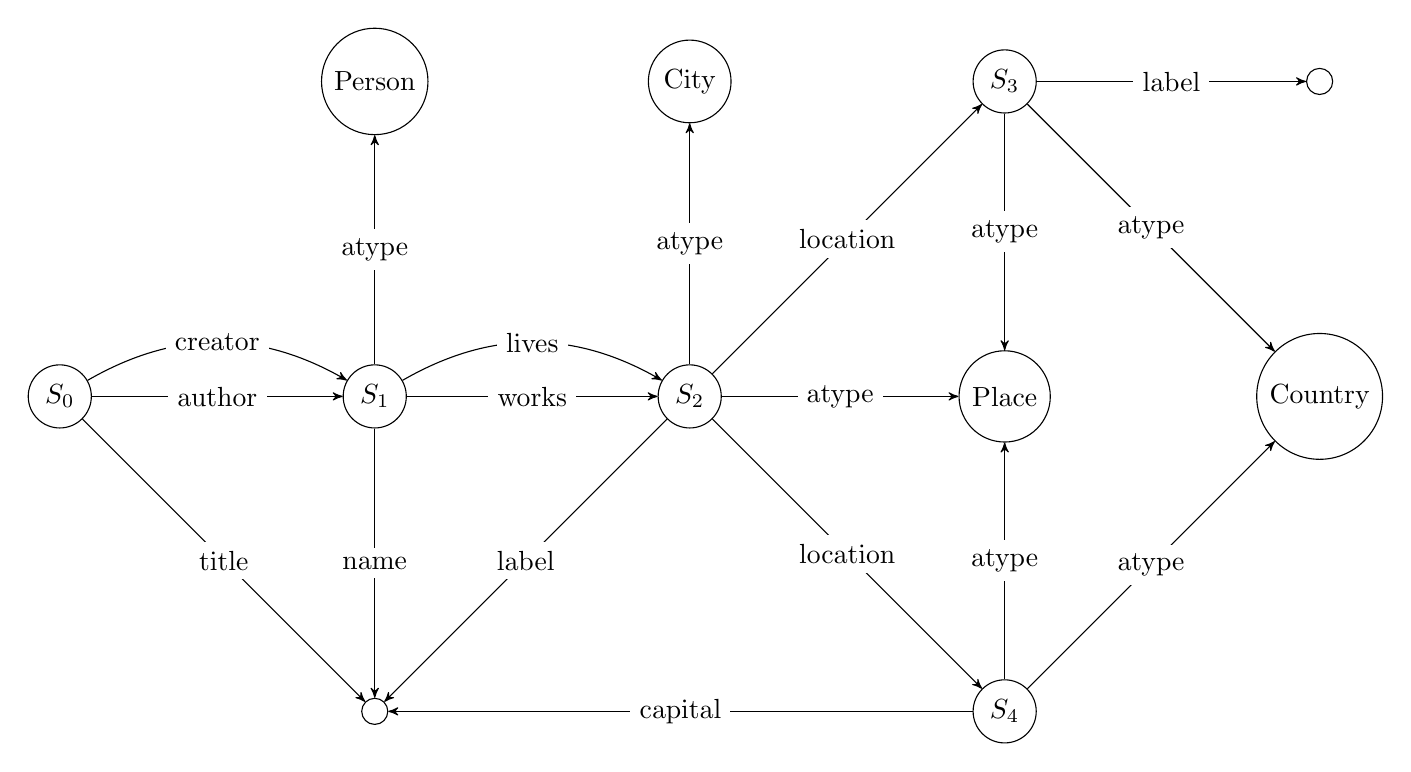
\begin{tikzpicture}[->,>=stealth',node distance=4cm]
\node [draw,circle] (n0) {$S_0$};
% \node (n0) [draw,thick,rectangle,inner sep=0] {
% \begin{tabular}{l}
% \multicolumn{1}{c}{$S_0$} \\
% \hline
% \\
% \hline
% - title
% \end{tabular}
% };

\node [draw,circle,right of = n0] (n1) {$S_1$};
% \node (n1) [draw,thick,rectangle,inner sep=0,right of = n0] {
% \begin{tabular}{l}
% \multicolumn{1}{c}{$S_1$} \\
% \hline
% - Person \\
% \hline
% - name
% \end{tabular}
% };

\node [draw,circle,above of = n1] (person) {Person};
\node [draw,circle,right of = n1] (n2) {$S_2$};
% \node (n2) [draw,thick,rectangle,inner sep=0,right of = n1] {
% \begin{tabular}{l}
% \multicolumn{1}{c}{$S_2$} \\
% \hline
% - City \\
% \hline
% - label
% \end{tabular}
% };

\node [draw,circle,right of = n2] (place) {Place};
\node [draw,circle,above of = place] (n3) {$S_3$};
% \node (n3) [draw,thick,rectangle,inner sep=0,above right of = n2] {
% \begin{tabular}{l}
% \multicolumn{1}{c}{$S_3$} \\
% \hline
% - Place \\
% - Country \\
% \hline
% - label
% \end{tabular}
% };

\node [draw,circle,above of = n2] (city) {City};
\node [draw,circle,below of = place] (n4) {$S_4$};
% \node (n4) [draw,thick,rectangle,inner sep=0,below right of = n2] {
% \begin{tabular}{l}
% \multicolumn{1}{c}{$S_4$} \\
% \hline
% - Place \\
% - Country \\
% \hline
% - capital
% \end{tabular}
% };

\node [draw,circle,right of = place] (country) {Country};
\node [draw,circle,below of = n1] (s1) {$\varnothing$};
\node [draw,circle,right of = n3] (s2) {$\varnothing$};

\path
(n0) edge node[fill=white] {author} (n1)
(n0) edge[bend left] node[fill=white] {creator} (n1)
(n1) edge node[fill=white] {\gls{atype}} (person)
(n1) edge node[fill=white] {works} (n2)
(n1) edge[bend left] node[fill=white] {lives} (n2)
(n2) edge node[fill=white] {\gls{atype}} (city)
(n2) edge node[fill=white] {location} (n3)
(n2) edge node[fill=white] {location} (n4)
(n2) edge node[fill=white] {\gls{atype}} (place)
(n3) edge node[fill=white] {\gls{atype}} (country)
(n4) edge node[fill=white] {\gls{atype}} (country)
(n3) edge node[fill=white] {\gls{atype}} (place)
(n4) edge node[fill=white] {\gls{atype}} (place)
(n0) edge node[fill=white] {title} (s1)
(n1) edge node[fill=white] {name} (s1)
(n2) edge node[fill=white] {label} (s1)
(n4) edge node[fill=white] {capital} (s1)
(n3) edge node[fill=white] {label} (s2)
;
\end{tikzpicture}
		}
	\end{minipage}
	\quad
	\begin{minipage}[h]{.2\textwidth}
		\centering
		\caption*{$R_a\left(V, \mathcal{W}\right)$}
		\resizebox{\textwidth}{!}{
		\begin{tabular}{lc@{\hs}l}
			\toprule
			$V$ & \phantom{a} & $\mathcal{W}$ \\
			\cmidrule{1-1} \cmidrule{3-3}
			$v_0$ & \phantom{a} & $S_0$ \\
			$v_1$, $v_2$ & \phantom{a} & $S_1$ \\
			$v_3$, $v_4$, $v_5$ & \phantom{a} & $S_2$ \\
			$v_6$ & \phantom{a} & $S_3$ \\
			$v_7$ & \phantom{a} & $S_4$ \\
			\bottomrule
		\end{tabular}}
	\end{minipage}
	\caption{Summary of the graph in Figure~\ref{fig:graph} with $R_a$. The table indicates the mappings by $R_a$. The content in $G$ is abstracted by the sumnode $\varnothing$.}
	\label{fig:attributes-summary}
\end{figure}
\vspace{.5cm}

\minisec{Summarisation Relation $R_{at}$}

We define $R_{at}$ as the relation that maps a node based on its set of types and attributes. We call the summary it generates the \emph{attributes \& types} summary.
The nodes $v_1$ and $v_2$ are mapped to a same sumnode by $R_{at}$ because they are associated with the same type, i.e., \emph{Person}, and they have the same attributes, i.e., $\left\lbrace lives, name, type, works \right\rbrace$.

\begin{definition}[Attributes \& Types Summary]
	Let $G=\left\langle V, A, l_V \right\rangle$ and $\mathcal{S}_{at} = \left\langle \mathcal{W}_{at}, \mathcal{B}_{at}, l_{\mathcal{W}_{at}} \right\rangle$ be two graphs.

	The set of nodes $\mathcal{W}_{at}$ is a subset of the source material disjoint from $V$, i.e., $\mathcal{W}_{at} \subseteq \mathcal{Z}$ with $V \cap \mathcal{W}_{at} = \emptyset$, and it contains as many elements as the power set of attributes and types in the graph:
	$$
	\begin{aligned}
	\lvert \mathcal{W}_{at} \rvert = \lvert \mathbb{P} ( & \{ \alpha \mid (u, v) \in V^2\; \exists (u, \alpha, v) \in A \} \;\cup \\
	& \{ l_V(c) \mid \exists (u, \glssymbol{atype}, c) \in A \wedge \glssymbol{atype} \in T \} ) \rvert
	\end{aligned}
	$$

	We call $\mathcal{S}_{at}$ the attributes \& types summary of $G$ according to the summarisation relation $R_{at} \subseteq V \times \mathcal{W}_{at}$ defined as:
	$$
	\begin{aligned}
	R_{at} = \{ (u, x) \in V \times \mathcal{W}_{at} \mid &\; types(u) = types(x) \\
	& \wedge attributes(u) = attributes(x) \}
	\end{aligned}
	$$
	\label{def:at}
\end{definition}

\minisec{Summarisation Relation $R_{ioa}$}

We define $R_{ioa}$ the relation based on the set of incoming and outgoing attributes. We call the summary it generates the \emph{IO attributes} summary.
All three nodes $v_3$, $v_4$, and $v_5$ map to the same sumnode by the relation $R_a$. However with $R_{ioa}$, each is assigned to a separate sumnode, since all three have different incoming set of attributes, i.e., $\left\lbrace lives \right\rbrace$, $\left\lbrace works \right\rbrace$, and $\varnothing$, respectively.

\begin{definition}[IO Attributes Summary]
	Let $G=\left\langle V, A, l_V \right\rangle$ and $\mathcal{S}_{ioa} = \left\langle \mathcal{W}_{ioa}, \mathcal{B}_{ioa}, l_{\mathcal{W}_{ioa}} \right\rangle$ be two graphs.

	The set of nodes $\mathcal{W}_{ioa}$ is a subset of the source material disjoint from $V$, i.e., $\mathcal{W}_{ioa} \subseteq \mathcal{Z}$ with $V \cap \mathcal{W}_{ioa} = \emptyset$, and it contains as many elements as the power set of attributes in the graph:
	$$
	\lvert \mathcal{W}_{ioa} \rvert = \lvert \mathbb{P}\left( \left\lbrace \alpha \mid (u, v) \in V^2\; \exists (u, \alpha, v) \in A \right\rbrace \right) \rvert
	$$

	We call $\mathcal{S}_{ioa}$ the IO attributes summary of $G$ according to the summarisation relation $R_{ioa} \subseteq V \times \mathcal{W}_{ioa}$ defined as:
	$$
	\begin{aligned}
	R_{ioa} =
	\{
	(u, x) \in V \times \mathcal{W}_{ioa} \mid &\; attributes(u) = attributes(x) \\
	& \wedge attributes^{-1}(u) = attributes^{-1}(x)
	\}
	\end{aligned}
	$$
	\label{def:ioa}
\end{definition}

\vspace{.5cm}

\minisec{Summarisation Relation $R_{ia}$}

We define $R_{ia}$ as the relation based on the set of incoming attributes. We call the summary it generates the \emph{incoming attributes} summary.

\begin{definition}[Incoming Attributes Summary]
	Let $G=\left\langle V, A, l_V \right\rangle$ and $\mathcal{S}_{ia} = \left\langle \mathcal{W}_{ia}, \mathcal{B}_{ia}, l_{\mathcal{W}_{ia}} \right\rangle$ be two graphs.

	The set of nodes $\mathcal{W}_{ia}$ is a subset of the source material disjoint from $V$, i.e., $\mathcal{W}_{ia} \subseteq \mathcal{Z}$ with $V \cap \mathcal{W}_{ia} = \emptyset$, and it contains as many elements as the power set of attributes in the graph:
	$$
	\lvert \mathcal{W}_{ia} \rvert = \lvert \mathbb{P}\left( \left\lbrace \alpha \mid (u, v) \in V^2\; \exists (u, \alpha, v) \in A \right\rbrace \right) \rvert
	$$

	We call $\mathcal{S}_{ia}$ the incoming attributes summary of $G$ according to the summarisation relation $R_{ia} \subseteq V \times \mathcal{W}_{ia}$ defined as:
	$$
	R_{ia} = \left\lbrace (u, x) \in V \times \mathcal{W}_{ia} \mid attributes^{-1}(u) = attributes^{-1}(x) \right\rbrace
	$$
	\label{def:ia}
\end{definition}

\begin{remark}
We note that the nodes that do not have any incoming attributes are mapped to the undefined sumnode $\mathfrak{U}$.
\end{remark}

\vspace{.5cm}

\minisec{Summarisation Relation $R_{iat}$}

We define $R_{iat}$ as the relation based on the set of types and incoming attributes. We call the summary this relation generates the \emph{incoming attributes \& types} summary.

\begin{definition}[Incoming Attributes \& Types Summary]
	Let $G=\left\langle V, A, l_V \right\rangle$ and $\mathcal{S}_{iat} = \left\langle \mathcal{W}_{iat}, \mathcal{B}_{iat}, l_{\mathcal{W}_{iat}} \right\rangle$ be two graphs.

	The set of nodes $\mathcal{W}_{iat}$ is a subset of the source material disjoint from $V$, i.e., $\mathcal{W}_{iat} \subseteq \mathcal{Z}$ with $V \cap \mathcal{W}_{iat} = \emptyset$, and it contains as many elements as the power set of attributes and types in the graph:
	$$
	\begin{aligned}
	\lvert \mathcal{W}_{iat} \rvert = \lvert \mathbb{P} ( & \{ \alpha \mid (u, v) \in V^2\; \exists (u, \alpha, v) \in A \} \;\cup \\
	& \{ l_V(c) \mid \exists (u, \glssymbol{atype}, c) \in A \wedge \glssymbol{atype} \in T \} ) \rvert
	\end{aligned}
	$$

	We call $\mathcal{S}_{iat}$ the incoming attributes \& types summary of $G$ according to the summarisation relation $R_{iat} \subseteq V \times \mathcal{W}_{iat}$ defined as:
	$$
	\begin{aligned}
	R_{iat} = \{ (u, x) \in V \times \mathcal{W}_{iat} \mid &\; types(u) = types(x) \\
	& \wedge attributes^{-1}(u) = attributes^{-1}(x) \}
	\end{aligned}
	$$
	\label{def:iat}
\end{definition}
\vspace{.5cm}

\minisec{Summarisation Relation $R_{ioat}$}

The relation $R_{ioat}$ maps a node based on the set of types, and the incoming and outgoing attributes sets. We call the summary this relation generates the \emph{IO attributes \& types} summary.
Although the nodes $v_1$ and $v_2$ are mapped to a same sumnode with $R_{at}$, that is not the case with the relation $R_{ioat}$, because only the node $v_2$ has the incoming attribute $creator$.
% With $R_{ioa}$ and $R_{ioat}$, the incoming set of attributes is computed by reversing the direction of edges, i.e., the target becomes the source, and then grouping on the source node.
%For these relations, the complexity is equal to $O\left(\vert A \vert\right)$, since we need to visit each edge in order to assign the node at the source of an edge to an equivalence class.

\begin{definition}[IO Attributes \& Types Summary]
	Let $G=\left\langle V, A, l_V \right\rangle$ and $\mathcal{S}_{ioat} = \left\langle \mathcal{W}_{ioat}, \mathcal{B}_{ioat}, l_{\mathcal{W}_{ioat}} \right\rangle$ be two graphs.

	The set of nodes $\mathcal{W}_{ioat}$ is a subset of the source material disjoint from $V$, i.e., $\mathcal{W}_{ioat} \subseteq \mathcal{Z}$ with $V \cap \mathcal{W}_{ioat} = \emptyset$, and it contains as many elements as the power set of attributes and types in the graph:
	$$
	\begin{aligned}
	\lvert \mathcal{W}_{ioat} \rvert = \lvert \mathbb{P} ( & \{ \alpha \mid (u, v) \in V^2\; \exists (u, \alpha, v) \in A \} \;\cup \\
	& \{ l_V(c) \mid \exists (u, \glssymbol{atype}, c) \in A \wedge \glssymbol{atype} \in T \} ) \rvert
	\end{aligned}
	$$

	We call $\mathcal{S}_{ioat}$ the IO attributes \& types summary of $G$ according to the summarisation relation $R_{ioat} \subseteq V \times \mathcal{W}_{ioat}$ defined as:
	$$
	\begin{aligned}
	R_{ioat} = \{ (u, x) \in V \times \mathcal{W}_{ioat} \mid &\; types(u) = types(x) \\
	& \wedge attributes(u) = attributes(x) \\
	& \wedge attributes^{-1}(u) = attributes^{-1}(x) \}
	\end{aligned}
	$$
	\label{def:ioat}
\end{definition}
\vspace{.5cm}

\begin{table}
	\centering
	\resizebox{\textwidth}{!}{
	\begin{tabular}{lc@{\hs}lc@{\hs}l}
	\toprule
	 & \phantom{a} & \multicolumn{1}{c}{Notation} & \phantom{a} & \multicolumn{1}{c}{Summarisation Relation} \\
	\cmidrule{3-3} \cmidrule{5-5}
	\emph{Single-Type} & \phantom{a} & $\mathcal{S}_{st} = \left\langle \mathcal{W}_{st}, \mathcal{B}_{st}, l_{\mathcal{W}_{st}} \right\rangle$ & \phantom{a} & Definition (\ref{def:st}) \\

	\emph{Types} & \phantom{a} & $\mathcal{S}_t = \left\langle \mathcal{W}_t, \mathcal{B}_t, l_{\mathcal{W}_t} \right\rangle$ & \phantom{a} & Definition (\ref{def:t}) \\

	\emph{Attributes} & \phantom{a} & $\mathcal{S}_a = \left\langle \mathcal{W}_a, \mathcal{B}_a, l_{\mathcal{W}_a} \right\rangle$ & \phantom{a} & Definition (\ref{def:a}) \\

	\emph{Attributes \& Types} & \phantom{a} & $\mathcal{S}_{at} = \left\langle \mathcal{W}_{at}, \mathcal{B}_{at}, l_{\mathcal{W}_{at}} \right\rangle$ & \phantom{a} & Definition (\ref{def:at}) \\

	\emph{IO Attributes} & \phantom{a} & $\mathcal{S}_{ioa} = \left\langle \mathcal{W}_{ioa}, \mathcal{B}_{ioa}, l_{\mathcal{W}_{ioa}} \right\rangle$ & \phantom{a} & Definition (\ref{def:ioa}) \\

	\emph{IO Attributes \& Types} & \phantom{a} & $\mathcal{S}_{ioat} = \left\langle \mathcal{W}_{ioat}, \mathcal{B}_{ioat}, l_{\mathcal{W}_{ioat}} \right\rangle$ & \phantom{a} & Definition (\ref{def:ioat}) \\

	\emph{Incoming Attributes} & \phantom{a} & $\mathcal{S}_{ia} = \left\langle \mathcal{W}_{ia}, \mathcal{B}_{ia}, l_{\mathcal{W}_{ia}} \right\rangle$ & \phantom{a} & Definition (\ref{def:ia}) \\

	\emph{Incoming Attributes \& Types} & \phantom{a} & $\mathcal{S}_{iat} = \left\langle \mathcal{W}_{iat}, \mathcal{B}_{iat}, l_{\mathcal{W}_{iat}} \right\rangle$ & \phantom{a} & Definition (\ref{def:iat}) \\

	\bottomrule
	\end{tabular}}
	\caption{Summarisation relations for approximate graph summaries}
	\label{tab:sumrel}
\end{table}

We note that the presented \emph{approximate} summarisation relations are indeed not precise, because they do not fulfill the Definition~\ref{def:precise-summary}. Indeed, it is possible to find a path in the approximate summary for which an instance as per Definition~\ref{def:summary-path-instance} does not form a path in the graph. For instance, the set $\{v_1, v_5, v_6\}$ is an instance of the summary path $works \cdot location \cdot capital$; however, there is no path that connects all three nodes $v_1$, $v_5$, and $v_6$ with the attributes $works$, $location$, and $capital$.
